\section{Méthode des moindres au carré}
\section{Approximation selon une droite de régression}
\subsection{Présentation}
Pour approximer une collection de points à l'aide d'une droite de régression, nous allons utiliser le cas particulier de la méthode des moindres au carré. Dans ce cas, l'approximation se fait par une droite représentative du polynôme $f(x)=a_0x+a_1$ et on obtient $a_0$ et $a_1$ par les calculs suivants:\vspace{6pt}\\
\begin{center}
        $a_0=\frac{\overline{y}\times\overline{x^2}-\overline{x}\times\overline{yx}}{\overline{x^2}-(\overline{x})^2},$\vspace{5pt}\\
        $a_1=\frac{\overline{yx}-\overline{x}\times\overline{y}}{\overline{x^2}-(\overline{x})^2}$
\end{center}
où $\overline{x}=\frac{\sum\limits_{i=0}^{n-1}x_i}{n}$, $\overline{yx}=\frac{\sum\limits_{i=0}^{n-1}x_iy_i}{n}$, $\overline{y}=\frac{\sum\limits_{i=0}^{n-1}y_i}{n}$, $\overline{x^2}=\frac{\sum\limits_{i=0}^{n-1}x_i^2}{n}$\vspace{4pt}\\
\subsection{Résolution manuelle}
Soient les points $(1,3), (8,1), (1.5, -1)$. Approximer ces points par une droite de régression.\\
Dans un premier temps, calculons $\overline{x}, \overline{y}, \overline{x^2}, \overline{yx}$:\\
\begin{center}
$\overline{x}=(1+8+1.5)/3=3.5$\vspace{3pt}\\
$\overline{y}=(3+1-1)/3=1$\vspace{3pt}\\
$\overline{x^2}=(1^2+8^2+1.5^2)/3\thickapprox22.42$\vspace{3pt}\\
$\overline{yx}=(1\times3+8\times1+1.5\times(-1))/3\thickapprox3.17$\vspace{3pt}\\
\end{center}
On calcule alors $a_0$ et $a_1$:\\
\begin{align*}
    a_0=\frac{1\times22.42-3.5\times3.17}{22.42-3.5^2}\thickapprox1.11\vspace{5pt}\\
    a_1=\frac{3.17-3.5\times1}{22.42-3.5^2}\thickapprox -0.03
\end{align*}
Ainsi, la droite d'équation $y=-0.03x+1.11$ approxime les points $(1,3), (8,1), (1.5, -1)$.
\newpage
\subsection{Algorithme et Implémentation en C}
\textit{\underline{Note: } pour l'implémentation de cette approximation, nous allons réutiliser la matrice de stockage des points, la structure \_polynom, ainsi que leurs fonctions associées (c.f. section \ref{header}).}\vspace{5pt}\\
Pour implémenter cette approche, nous avons donc besoin de calculer les moyennes blablabla . Pour cela, nous avons implémenté une fonction \textbf{getMeans}. Voici son pseudo-code:\\
\begin{lstlisting}[mathescape=true, basicstyle=\fontsize{8}{10}\selectfont]
Fonction getMeans:
    sumX = 0
    sumY = 0
    sumX2 = 0
    sumXY = 0;
    Pour i de 0 a n:
        sumX$+=x_i$
        sumY$+=y_i$
        sumX2$+=x_i \times x_i$
        sumXY$+=x_i + y_i$
    renvoyer $[\frac{sumX}{nbPoints}, \frac{sumY}{nbPoints}, \frac{sumX2}{nbPoints}, \frac{sumXY}{nbPoints}]$
\end{lstlisting}
Ceci fait, ils nous reste simplement à coder la fonction qui retourne le bon polynôme. Voici son implémentation en C:\\
\begin{lstlisting}[mathescape=true, basicstyle=\fontsize{8}{10}\selectfont]
_polynom computeLinearPolynom(float** data, int n) {
    _polynom polynom = createPolynom(1);
    float* meanValues = getMeans(data, n);
    polynom.coefficients[0] = ((meanValues[1] * meanValues[2]) - (meanValues[0] * meanValues[3])) /
                                    (meanValues[2] - (meanValues[0] * meanValues[0]));
    polynom.coefficients[1] = (meanValues[3] - (meanValues[0] * meanValues[1])) /
                                    (meanValues[2] - (meanValues[0] * meanValues[0]));
    
    free(meanValues);
    return polynom;
}
\end{lstlisting}
Nous ne détaillerons pas ici les fonctions d'affichage telles que les fonctions pour afficher une matrice ou pour afficher un polynôme.
\newpage
\subsection{Exemples d'exécutions et graphiques}
Vous trouverez en annexe de ce rapport plusieurs jeux de données qui peuvent être approximés par une droite. C'est notamment le cas des 3 premiers. Voici les polynômes retournés par l'exécution du programme avec ces collections, ainsi que la représentation graphique illustrant les résultats.\\
\textbf{Premier Jeu de Données}\\
Après exécution, notre programme retourne le polynôme: $y=-0.000186x+1.001279$. Nous avons tracé le polynôme ainsi que les points fournis pour obtenir le graphique suivant:\\
\begin{figure}[H]
    \centering
    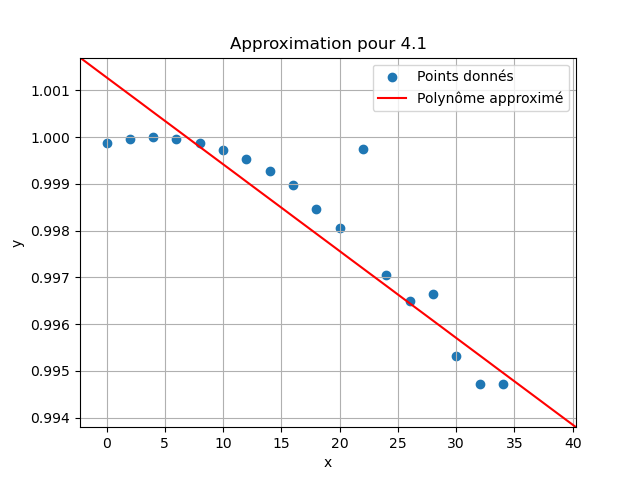
\includegraphics[width=0.6\textwidth]{sources/Corentin/approximationC/results/graphs/41.png}
    \caption{Approximation du premier jeu de données}
\end{figure}
\textbf{Deuxième Jeu de Données}\\
Après exécution, notre programme retourne le polynôme: $y=0.324356x+-112.658463$. Nous avons tracé le polynôme ainsi que les points fournis pour obtenir le graphique suivant:\\
\begin{figure}[H]
    \centering
    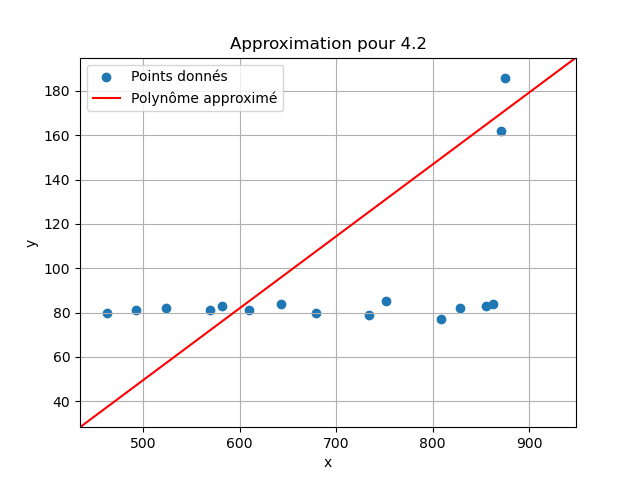
\includegraphics[width=0.6\textwidth]{sources/Corentin/approximationC/results/graphs/42.png}
    \caption{Approximation du deuxième jeu de données}
\end{figure}
\newpage
\textbf{Troisième Jeu de Données}\\
Après exécution, notre programme retourne le polynôme: $y=0.500092x+3.000079$. Nous avons tracé le polynôme ainsi que les points fournis pour obtenir le graphique suivant:\\
\begin{figure}[h]
    \centering
    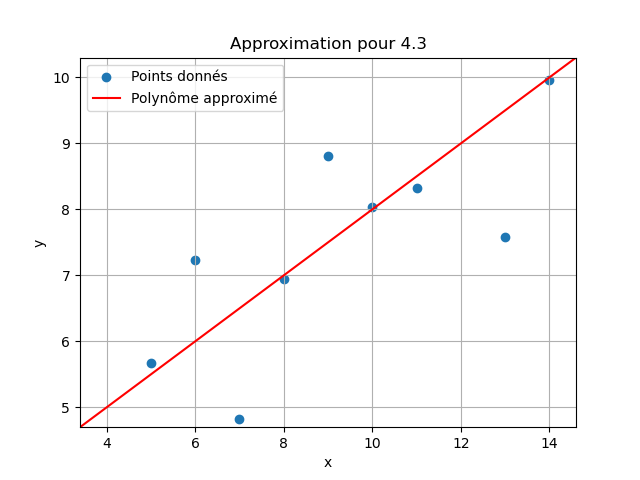
\includegraphics[width=0.6\textwidth]{sources/Corentin/approximationC/results/graphs/43.png}
    \caption{Approximation du deuxième jeu de données}
\end{figure}
\newpage
\section{Approximation selon un ajustement exponentiel}
\subsection{Présentation}
L'objectif pour nous ici va être de trouver un moyen de revenir à une regression linéaire. Pour cela, il faut que l'on retrouve une forme $y=ax+b$ en partant d'une forme $y=ce^{dx}$. En manipulant l'expression grâce à l'exponentielle et au logarithme népérien, nous obtenons le résultat suivant: \\
\begin{center}
    \begin{align*}
        y&=ce^{dx}\\
        ln(y)&=ln(ce^{dx})\\
        ln(y)&=ln (c)+ dx \\
    \end{align*}
\end{center}
On pose $Y=ln(y)$, $B=ln(c)$ et $A=d$. On peut alors écrire $Y=Ax+B$. C'est la forme que l'on souhaitait.
À partir des points initiaux, nous allons calculer $z_i=ln(y_i)$ pour $i=0,..., n-1$. Il suffira alors de calculer une droite de régression comme vue précedemment avec les points $(x_i, z_i)$. Enfin, nous calculerons la valeur de $c$ et $d$ avec ce qui a été posé précedemment pour obtenir une forme exponentielle. 
\subsection{Résolution manuelle}
Soient les points $(2,1), (3,4), (2.5, 3)$. Approximer ces points par un ajustement exponentiel.\\
Calculons $z_i=ln(y_i)$ pour $i=0,1,2$:\\
\begin{center}
    \begin{align*}
        z_0&=ln(y_0)=ln(1)=0\\
        z_1&=ln(y_1)=ln(4)\thickapprox1.39\\
        z_2&=ln(y_2)=ln(3)\thickapprox 1.1\vspace{4pt}\\
    \end{align*}
\end{center}
Calculons alors une droite de régression qui approxime tous les points $(x_i, z_i)$:\\
Après calculs, nous obtenons: \\
\begin{center}
    $\overline{x}=2.5$\vspace{3pt}\\
    $\overline{z}\thickapprox0.83$\vspace{3pt}\\
    $\overline{x^2}\thickapprox6.42$\vspace{3pt}\\
    $\overline{zx}\thickapprox2.31$\vspace{3pt}\\
\end{center}
Nous pouvons alors calculer $B$ et $A$, pour obtenir la droite $Y=1.38x-2.63$.
Enfin, il ne nous reste plus qu'à exprimer la forme exponentielle, en faisant le chemin inverse que celui qui est présenté au début de cette partie.\\
\begin{center}
    \begin{align*}
        Y&=Ax+B=1.38x-2.63\\
        \Leftrightarrow ln(y)&=ln (c)+ dx \\
        \Leftrightarrow y&=e^{ln(c)+dx}=e^{ln(c)}\times e^{dx}=e^{-2.63}\times e^{1.38x}=0.072e^{1.38x}\\
    \end{align*}
\end{center}
Nous avons donc comme approximation exponentielle $y=0.072e^{1.38x}$.
\subsection{Algorithme et Implémentation en C}
\textit{\underline{Note: } pour l'implémentation de cette approximation, nous allons réutiliser la matrice de stockage des points, la structure \_polynom, ainsi que leurs fonctions associées (c.f. section \ref{header}). Nous réutiliserons également la fonction getMeans vu précédemment.}\vspace{5pt}\\
Pour implémenter cette approximation, nous allons devoir créer une deuxième matrice de points, qui cette fois contiendra les points $(x_i, ln(y_i))$. Pour cela, nous allons coder une fonction \textit{completeDataMatrix}, qui sera par ailleurs réutilisée dans l'approximation par un ajustement de puissance. Cette fonction va prendre en paramètre la matrice de donnée initiale, une nouvelle matrice de donnée vierge, le nombre de points donnés, et le type d'approximation (exponentiel ou puissance). Voici son implémentation en C :\\
\begin{lstlisting}[mathescape=true, basicstyle=\fontsize{8}{10}\selectfont]
    void completeDataMatrix(float** data, float** matrix, int nbData, char type){
        for (int i = 0; i < nbData; i++) {
            if(type=='e'){
                matrix[0][i]=data[0][i];
                matrix[1][i]=logf(data[1][i]);
            }
            ...
        }
    }       
\end{lstlisting}
À partir de là, nous avons tous les outils nécessaires pour l'approximation. Voici le code source de la fonction qui calcule le polynôme recherché:\\
\begin{lstlisting}[mathescape=true, basicstyle=\fontsize{8}{10}\selectfont]
_polynom computeExponentialPolynom(float** data, int n) {
    //Creation d'une matrice pour les donnees necessaires a l'ajustement exponentiel
    float** dataForExp = createMatrix(2, n);
    completeDataMatrix(data, dataForExp, n, 'e');
    //Creation du polynome ln(y)=Bx+A
    _polynom polynom = computeLinearPolynom(dataForExp, n);
    //Transformation en y=exp(A)exp(Bx)
    polynom.coefficients[0]=expf(polynom.coefficients[0]);
    polynom.coefficients[1]=polynom.coefficients[1];
    freeMatrix(dataForExp, 2);
    return polynom;
}
\end{lstlisting}
\newpage
\subsection{Exemples d'exécutions et graphiques}
Pour mettre en pratique le code précédemment présenté, nous pouvons l'exécuter avec le quatrième jeu de donnée présent en annexe du rapport. En effet, les points se pretent bien à une approximation exponentielle.\\
Voici le polynôme retourné par le programme: $y=0.000020exp(0.143061x)$. Nous avons tracé le polynôme ainsi que les points fournis pour obtenir le graphique suivant:\\
\begin{figure}[H]
    \centering
    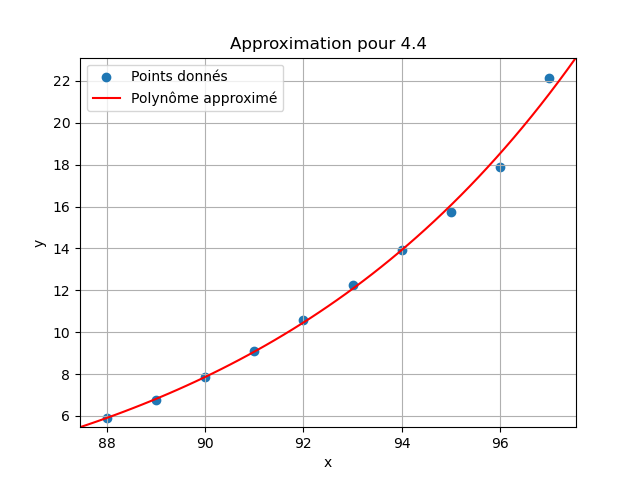
\includegraphics[width=0.6\textwidth]{sources/Corentin/approximationC/results/graphs/44.png}
    \caption{Approximation du quatrième jeu de données}
\end{figure}
\section{Approximation selon un ajustement puissance}
\subsection{Présentation}
Le but va ici être de trouver un moyen de revenir à une regression linéaire, de la même manière que pour l'approximation exponentielle. Pour cela, il faut que l'on retrouve une forme $y=ax+b$ en partant d'une forme $y=ax^b$. En manipulant l'expression grâce au logarithme, nous obtenons le résultat suivant: \\
\begin{center}
    \begin{align*}
        y&=ax^b\\
        log(y)&=log(ax^b)\\
        log(y)&=log(a)+blog(x) \\
    \end{align*}
\end{center}
On pose $Y=ln(y)$, $B=log(a)$, $A=b$ et $X=log(x)$. On peut alors écrire $Y=AX+B$. C'est la forme que l'on souhaitait.
À partir des points initiaux, nous allons calculer $w_i=log(x_i)$ et $z_i=log(y_i)$ pour $i=0,..., n-1$. Il suffira alors de calculer une droite de régression comme vue précedemment avec les points $(w_i, z_i)$. Enfin, nous calculerons la valeur de $a$ et $b$ avec ce qui a été posé précedemment pour obtenir un ajustement puissance. 
\newpage
\subsection{Résolution manuelle}
Soient les points $(1,3), (2,7), (5, 1.3)$. Approximer ces points par un ajustement puissance.\\
Calculons $w_i=log(x_i)$ et $z_i=log(y_i)$ pour $i=0,1,2$:\\
\begin{center}
    D'une part: 
    \begin{align*}
        w_0&=log(x_0)=log(1)=0\\
        w_1&=log(x_1)=log(2)\thickapprox0.3\\
        w_2&=log(x_2)=log(5)\thickapprox 0.7\vspace{2pt}\\
    \end{align*}
    D'autre part: 
    \begin{align*}
        z_0&=log(y_0)=log(3)\thickapprox0.48\\
        z_1&=log(y_1)=log(7)\thickapprox0.84\\
        z_2&=log(y_2)=log(1.3)\thickapprox 0.11\vspace{2pt}\\
    \end{align*}
\end{center}
Calculons alors une droite de régression qui approxime tous les points $(w_i, z_i)$:\\
Après calculs, nous obtenons: \\
\begin{center}
    $\overline{w}=0.34$\vspace{3pt}\\
    $\overline{z}\thickapprox0.48$\vspace{3pt}\\
    $\overline{w^2}\thickapprox0.19$\vspace{3pt}\\
    $\overline{wz}\thickapprox0.11$\vspace{3pt}\\
\end{center}
Nous pouvons alors calculer $B$ et $A$, pour obtenir la droite $Y=-0.71x+0.71$.
Enfin, il ne nous reste plus qu'à exprimer le polynôme, en faisant le chemin inverse que celui qui est présenté au début de cette partie.\\
\begin{center}
    \begin{align*}
        Y&=Ax+B=-0.71x+0.71\\
        \Leftrightarrow log(y)&=log(a)+blog(x)\\
        \Leftrightarrow y&=10^{log(a)+blog(x)}=10^{log(a)}\times 10^{blog(x)}=10^{0.71}\times x^{-0.71}=5.12x^{-0.71}\\
    \end{align*}
\end{center}
Nous avons donc comme approximation exponentielle $y=5.12x^{-0.71}$.
\newpage
\subsection{Algorithme et Implémentation en C}
\textit{\underline{Note: } pour l'implémentation de cette approximation, nous allons réutiliser la matrice de stockage des points, la structure \_polynom, ainsi que leurs fonctions associées (c.f. section \ref{header}). Nous réutiliserons également la fonction getMeans et la fonction completeDataMatrix vues précédemment.}\vspace{5pt}\\
Pour implémenter cette approximation, nous allons aussi devoir créer une deuxième matrice de points, qui cette fois contiendra les points $(log(x_i), log(y_i))$. Pour cela, nous allons compléter la fonction \textit{completeDataMatrix}. Voici son implémentation en C :\\
\begin{lstlisting}[mathescape=true, basicstyle=\fontsize{8}{10}\selectfont]
    void completeDataMatrix(float** data, float** matrix, int nbData, char type){
        for (int i = 0; i < nbData; i++) {
            ...
            if(type=='p'){
                matrix[0][i] = log10f(data[0][i]);
                matrix[1][i] = log10f(data[1][i]);
            }
        }
    }       
\end{lstlisting}
À partir de là, nous avons tous les outils nécessaires pour l'approximation. Voici le code source de la fonction qui calcule le polynôme recherché:\\
\begin{lstlisting}[mathescape=true, basicstyle=\fontsize{8}{10}\selectfont]
_polynom computePowerPolynom(float** data, int n) {
    //Creation d'une matrice pour les donnees necessaires a l'ajustement puissance
    float** dataForPow = createMatrix(2, n);
    completeDataMatrix(data, dataForPow, n, 'p');
    //Creation du polynome log(y)=Blog(x)+A
    _polynom polynom = computeLinearPolynom(dataForPow, n);
    //Transformation en y=(10^A)x^B
    polynom.coefficients[0]=pow(10, polynom.coefficients[0]);
    polynom.coefficients[1]=polynom.coefficients[1];
    freeMatrix(dataForPow, 2);
    return polynom;
}
\end{lstlisting}
\newpage
\subsection{Exemples d'exécutions et graphiques}
Pour mettre en pratique le code précédemment présenté, nous pouvons l'exécuter avec le dernier jeu de donnée présent en annexe du rapport. En effet, les points se prêtent bien à une approximation polynomiale.\\
Voici le polynôme retourné par le programme: $y=696595.051263x^-2.527187$. Nous avons tracé le polynôme ainsi que les points fournis pour obtenir le graphique suivant:\\
\begin{figure}[H]
    \centering
    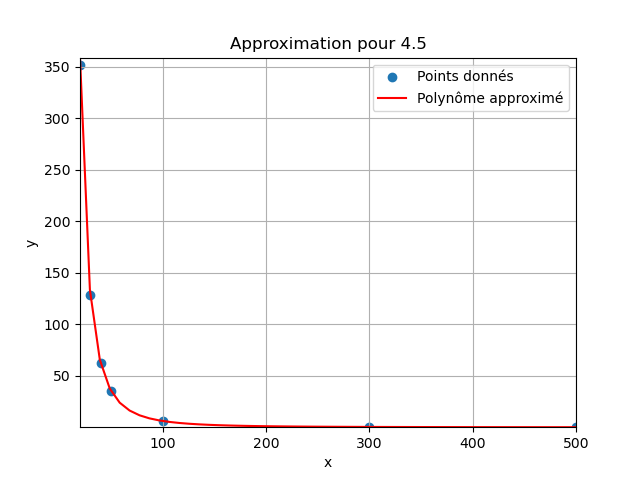
\includegraphics[width=0.6\textwidth]{sources/Corentin/approximationC/results/graphs/45.png}
    \caption{Approximation du cinquième jeu de données}
\end{figure}

